\providecommand{\main}{../../..}
\documentclass[\main/dresen_thesis.tex]{subfiles}
\renewcommand{\thisPath}{\main/chapters/theoreticalBackground/scattering}
\begin{document}
\section{Scattering}\label{sec:theoreticalBackground:scattering}
Scattering describes the general physical process, where radiation changes its straight path due to interaction with another object.
In a broad perspective this includes all various types of radiation - light, x-ray, electron, neutron, \etc .
For example it includes the very daily process of seeing, where after a light wave is emitted from a source like the sun or a light bulb, the wave is scattered from an object in the room before it is finally detected within ones eye. 
And scattering also includes the process where after a neutron is generated in a nuclear reactor, it interacts with a sample in a experimental hall before it is measured with a sophisticated detector.

In this work, multiple x-ray and neutron scattering techniques are applied to study the nuclear and magnetic structure of nanoparticles and their manufactured assemblies. 
To understand the rich information that is obtained by those techniques, \refsec{sec:theoreticalBackground:scattering:scatteringTheory} presents in the following a brief introduction to the general scattering theory and \refsec{sec:theoreticalBackground:scattering:interactionWithMatter} to the interaction of x-ray and neutrons with matter.
Then the theory behind the mainly applied techniques are discussed: small-angle scattering (\refsec{sec:theoreticalBackground:scattering:SASNanoparticles}), grazing-incidence small-angle scattering (\refsec{sec:theoreticalBackground:scattering:GISAS}) and reflectometry (\refsec{sec:theoreticalBackground:scattering:reflectometry}).
\subsection{Scattering Theory}\label{sec:theoreticalBackground:scattering:scatteringTheory}
In quantum mechanics, scattering theory describes the scattering of particles, \textit{e.g.} neutrons or x-ray photons, from a scattering center as depicted in \reffig{fig:theoreticalBackground:scattering:scatteringTheory:scatteringProcess}. An incoming wave $\vec{k}_i$ with defined direction can interact with a scattering center and due to this deviate from its straight path, exiting as outgoing wave $\vec{k}_o$. 
If energy is conserved ($|\vec{k}_i| = |\vec{k}_o|$) the process is called elastic and otherwise inelastic.
The vector describing the change from one momentum to the other is noted by
\begin{align}
  \vec{q} \eq \vec{k}_o - \vec{k}_i.
\end{align}
For an elastic process the magnitude of $\vec{q}$ is directly determined by the wavelength $\lambda$ and angle $2\theta$ between $\vec{k}_i$ and $\vec{k}_o$ by
\begin{align}
  |\vec{q}| \eq \frac{4 \pi}{\lambda} \sin(\theta),
\end{align}
where it is used that $|\vec{k}_i| = \frac{2 \pi}{\lambda}$.

\begin{figure}[tb]
  \centering
  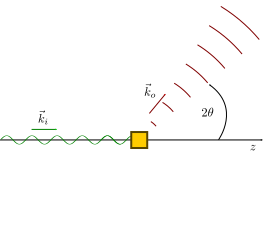
\includegraphics{scatteringTheory_scatterProcess}
  \caption{\label{fig:theoreticalBackground:scattering:scatteringTheory:scatteringProcess}General scattering process. An incoming wave with wave vector $\vec{k}_i$ (green) interacts with a scattering center (yellow) and produces an outgoing wave with wave vector $\vec{k}_o$ (red).}
\end{figure}

Scattering theory determines the transition probabilities for an particle to go from an incoming state to an outgoing state - respectively defined by their energy, momentum and polarization - in dependence of the properties of the particles, the scattering center and their interaction potential.
Thereby it provides a method to calculate from a model the expected scattering intensity, which can be compared to an actual scattering experiment.
Considering only non-relativistic physics, the problem that needs to be solved for this is the Schr\"odinger equation
\begin{align}
  \label{eq:theoreticalBackground:scattering:scatteringTheory:schrodingerEquation}
  \bigg(\frac{\hat{p}^2}{2m} + V \bigg) \ket{\psi} \eq E \ket{\psi},
\end{align}
with the boundary condition $V(\vec{r}) \eq 0$ for $\vec{r}$ outside the scattering region. In quantum mechanics, it is assumed that the scattering particles are non-interacting among themselves, which is a well approximation for photons and neutrons. 
The interaction between the wave and the scattering center is described completely by $V(\vec{r})$ and is discussed in further detail in \refsec{sec:theoreticalBackground:scattering:interactionWithMatter}. 
To solve \refeq{eq:theoreticalBackground:scattering:scatteringTheory:schrodingerEquation}, one defines the Hamiltonians
\begin{align}
  H_0 &\eq \frac{\hat{p}^2}{2m},\\
  H &\eq H_0 + V,
\end{align}
and defines $\ket{\phi}$ as the eigenstates of the free Schr\"odinger equation
\begin{align}
  H_0 \ket{\phi} &\eq E \ket{\phi}.\\
\end{align}
Now, naively, the Schr\"odinger equation can be rearranged as
\begin{align}
  \ket{\psi} &\eq \frac{1}{E - H_0} V \ket{\psi},
\end{align}
but this would not fulfil the boundary condition for $r \rightarrow \infty$, where $V\eq0$, and it has an ill-defined denominator for the eigenstates. 
Therefore, the correct solution needs the addition of the free particle solution and a definition how the pole is supposed to be treated. 
The latter is done by adding a infinitely small and positively complex value $i\epsilon$ to the denominator. The resulting equation
\begin{align}
  \ket{\psi} &\eq \ket{\phi} +  \frac{1}{E - H_0 + i \epsilon} V \ket{\psi},
\end{align}
is known as the Lippmann-Schwinger equation and  it solves the Schr\"odinger equation by construction. 
In position space, it reads as integral equation
\begin{align}
  \psi (\vec{r}) &\eq \phi(\vec{r}) + \int \dint \vec{r}^\prime \bra{\vec{r}}\frac{1}{E - H_0 + i \epsilon} \ket{\vec{r}^\prime} V (\vec{r}^\prime)\psi (\vec{r}^\prime),
  \label{eq:theoreticalBackground:scattering:scatteringTheory:LippmanSchwingerIntegralEquation}
\end{align}
where it is used that the single-particle potential is diagonal in position space $\bra{\vec{r}} V \ket{\vec{r}^\prime} = V(\vec{r}) \delta(\vec{r} - \vec{r}^\prime)$. 
The simplest solution for the free Hamiltonian is given by a plane wave
\begin{align}
  \phi_{\vec{k}}(\vec{r}) \eq e^{i\vec{k} \cdot \vec{r}}.
\end{align}
As a plane wave extends infinitely in space with constant amplitude, plane waves are not normalizable.
To describe physical particles with finite width, a superposition of plane waves can be used
\begin{align}
  \varphi(\vec{r}) \eq \frac{1}{\sqrt{2 \pi}^3} \int \dint \vec{k} \hat{\varphi} (\vec{k}) \phi_{\vec{k}}(\vec{r}),
\end{align}
where $\hat{\varphi} (\vec{k})$ describes the probability amplitude for a momentum $\vec{k}$ and is essentially the Fourier transform of $\varphi(\vec{r})$. 
However, as there is no term that couples momenta $\vec{k}$ and $\vec{k}^\prime$, it is sufficient to solve the Schr\"odinger equation just for a single plane wave and form the wave packet in the end.

The matrix element within the integral equation \refeq{eq:theoreticalBackground:scattering:scatteringTheory:LippmanSchwingerIntegralEquation} can be solved straight-forward in momentum space using the residue theorem as shown in \refapp{ch:appendix:calculations:greenFunctionFreeHamiltonian} and results in
\begin{align}
  \bra{\vec{r}}\frac{1}{E - H_0 + i \epsilon} \ket{\vec{r}^\prime} \eq -\frac{m}{2 \pi \hbar^2} \frac{e^{ik|\vec{r} - \vec{r}^\prime|}}{|\vec{r} - \vec{r}^\prime|}.
\end{align}
Thus the integral representation of the Lippmann-Schwinger equation is
\begin{align}
  \psi (\vec{r}) &\eq e^{i\vec{k} \cdot \vec{r}} - \frac{m}{2 \pi\hbar^2} \int \dint \vec{r}^\prime \frac{e^{ik|\vec{r} - \vec{r}^\prime|}}{|\vec{r} - \vec{r}^\prime|} V (\vec{r}^\prime)\psi (\vec{r}^\prime).
\end{align}
The resulting wave function can be nicely interpret as a sum of the incoming plane wave and the scattered wave, which is itself a superposition of spherical waves generated at $\vec{r}^\prime$ and that is modulated by the interaction potential $V(\vec{r}^\prime)$ and the wave field at this point.

In a standard experimental setup, the detector is often at a position that is far away relative to the scattering volume $r^\prime \ll r$. 
Therefore a good approximation and large simplification in calculation is
\begin{align}
  |\vec{r} - \vec{r}^\prime| \eq& r - \frac{\vec{r} \cdot \vec{r}^\prime}{r} + \mathcal{O}\bigg(\frac{{r^\prime}^2}{r}\bigg),\\
  \frac{1}{|\vec{r} - \vec{r}^\prime|} \eq& \frac{1}{r} + \mathcal{O}\bigg(\frac{r^\prime}{r^2} \bigg),\\
  \vec{k}^\prime \eq& k \vec{r} / r,
\end{align}
where the latter reads that as the detector is far away relative to the sample size, the outgoing wave points essentially into the direction of the detector. 
Then the Lippmann-Schwinger equation reads
\begin{align}
  \psi (\vec{r}) &\eq e^{i\vec{k} \cdot \vec{r}} - \frac{m}{2 \pi\hbar^2} \frac{e^{ikr}}{r} \int \dint \vec{r}^\prime e^{-i\vec{k} \cdot \vec{r}^\prime} V (\vec{r}^\prime)\psi (\vec{r}^\prime),
\end{align}
and the scattered wave only reads as a single spherical wave $e^{ikr} / r$ with an amplitude determined by the interaction of the wave function with the scattering center potential.

The Lippmann-Schwinger equation can be used to solve the scattering problem for any potential $V$ iteratively by starting on the right hand side of the equation with the free particle solution for $\psi (\vec{r})$ and then putting the solution back into the Lippmann-Schwinger equation, \etc.
The first iteration 
\begin{align}
  \psi (\vec{r}) &\eq e^{i\vec{k} \cdot \vec{r}} - \frac{m}{2 \pi\hbar^2} \frac{e^{ikr}}{r} \int \dint \vec{r}^\prime e^{-i\vec{q} \cdot \vec{r}^\prime} V (\vec{r}^\prime),
  \label{eq:theoreticalBackground:scattering:scatteringTheory:firstBornApproximation}
\end{align}
is known as the Born approximation and is the starting point for many further calculations. It fully describes the case where the wave undergoes only a single scattering event as it passes through the sample. 

Finally, one can determine from the wave function for an incoming flux of particles, the flux of scattered particles to a solid angle $\dint \Omega$, which is an experimentally accessible quantity.  The probability current of a wave function $\psi$  is calculated in quantum mechanics by
\begin{align}
  \vec{j} \eq \frac{\hbar}{2mi} \bigg( \psi^* \vec{\nabla} \psi - \psi \vec{\nabla} \psi^* \bigg).
\end{align}
Thus the incoming current and scattered current is evaluated to be
\begin{align}
  \vec{j}_i &\eq \frac{\hbar \vec{k}}{m}\\
  \vec{j}_o &\eq \bigg| \frac{m}{2 \pi\hbar^2} \int \dint \vec{r}^\prime e^{-i\vec{q} \cdot \vec{r}^\prime} V (\vec{r}^\prime) \bigg|^2 \frac{\hbar k}{m r^2} \hat{r} + \mathcal{O} \bigg(\frac{1}{r^3}\bigg),\\
\end{align}
and with this the incoming flux per unit area is determined to $\Phi_i \eq \vec{j}_i \cdot \hat{k}$, and the scattered flux per surface area to $\Phi_o \eq \vec{j}_o \cdot \dint \vec{S}$, where $\dint \vec{S} \eq r^2 \dint \Omega \hat{r}$. 
Experimentally one measures the flux of scattered particles to a solid angle and normalizes this to the corresponding flux of incoming particles. This ratio is known as the differential cross section and plugging in the previous results, it is calculated in Born approximation via
\begin{align}
  \frac{\dint \sigma}{\dint \Omega} \eq \frac{\Phi_o}{\Phi_i \dint \Omega} \eq \bigg| \frac{m}{2 \pi\hbar^2} \int \dint \vec{r}^\prime e^{-i\vec{q} \cdot \vec{r}^\prime} V (\vec{r}^\prime) \bigg|^2.
  \label{eq:theoreticalBackground:scattering:scatteringTheory:differentialCrossSectionBornApproximation}
\end{align}

\subsection{Interaction of X-rays and Neutrons with Matter}\label{sec:theoreticalBackground:scattering:interactionWithMatter}
To solve the Lippmann-Schwinger equation it is necessary to know how the scattering wave and the sample interact with each other, which is represented by the potential $V$.
In the case of x-rays, the dominant coupling to consider is the interaction of the x-ray photons with the electron shells of the atoms making up the material.
For neutrons the coupling to the electrons is negligible in contrast to the interaction with the nucleus of the atoms, but the additional degree of freedom coming from the magnetic moment of the neutron has to be considered, which introduces additional scattering contributions from the magnetic structure of the material.
In the following both interactions and how to evaluate them for different materials is presented briefly. 
Especially the magnetic scattering of the neutron is a topic that needs a more rigorous discussion that is skipped in the framework of this thesis and can instead be found in literature works like [].%INSERT REFERENCE

Neutrons scatter for one on the nuclei of the atoms of a material and additionally with their magnetic moments on the unpaired electrons in the electron shell of the atom. For the nuclear scattering, the wavelength of thermal neutrons $\mathcal{O} (10^{-10} \unit{m})$ is much larger than the the length scale of a nucleus ($\mathcal{O} (10^{-15} \unit{m})$. The nucleus can therefore be considered point-like. Additionally the scattering is considered to be spherically symmetric and thus the potential for the scattering of a free neutron from a single nucleus can be modelled by a Fermi pseudopotential
\begin{align}
  V(r) \eq \frac{2 \pi \hbar^2}{m} b \delta(r),
\end{align}
where $b$ is the coherent neutron scattering length, which is different for every element and isotope and includes thus the crucial information to differentiate between them. The \textit{ab initio} calculation of the scattering length for an isotope is a hard task, as it includes \textit{e.g.} resonance effects, which needs detailed knowledge of the subatomic structure. However, the experimental values have been tabulated for every isotope.

\subsection{Coherence \& Instrumental Resolution}\label{sec:theoreticalBackground:scattering:CoherenceInstrumentalResolution}
Also important
\subsection{Small-Angle Scattering from Nanoparticles}\label{sec:theoreticalBackground:scattering:SASNanoparticles}
Small-angle scattering is a technique to study nanometer sized objects when the wavelength of the scattered particle is in the order of a few {\aa}ngstr\"om. 
Here, the forward scattering of a collimated beam through a sample is measured on a position sensitive detector around an opening angle in the order of $2 \theta \eq 0.1^\circ - 10^\circ$. 
As the magnitude of the scattering vector $q$ is proportional to $\sin(\theta)$ and $q$ is inversely proportional to the probed length scale, smaller scattering angles $\theta$ mean that larger length scales are probed. 

In the following, the application of small-angle scattering to the study of nanoparticles in dispersion is described. 
In a first step, a dispersion that consists of monodisperse and equally oriented nanoparticles is considered. 
The potential $V(\vec{r})$ in the Born approximation formula of the differential cross section in \refeq{eq:theoreticalBackground:scattering:scatteringTheory:differentialCrossSectionBornApproximation} can be written as the sum of a constant background $V_m$ for the solvent and a position dependant potential for the nanoparticles $V_{np}$ in the solvent. The nanoparticle potential can be further rewritten as convolution of a potential $V_{p}(\vec{r})$ describing a single nanoparticle in the solvent and a function $s(\vec{r})$ describing the position of the $N$ nanoparticles in the solution. In total, we get
\begin{align}
  V(\vec{r}) \eq V_{m} + (s * V_{p})(\vec{r}),\\
  s(\vec{r}) \eq \sum_{j=1}^N \delta(\vec{r} - \vec{r}_j).
\end{align}
Inserting this potential into the Born approximation, the integral over the constant potential $V_m$ essentially vanishes\footnote{
  $\int \dint \vec{r} e^{-i \vec{q} \cdot \vec{r}} V_m \eq (2\pi)^3 V_m \delta(\vec{q})$ is zero for $\vec{q} \neq 0$, and describes forward scattering otherwise.
} and the convolution theorem turns the integral over the convolution to a product of two integrals
\begin{align}
  \bigg| \int \dint \vec{r} e^{-i\vec{q} \cdot \vec{r}} (s * V_{p})(\vec{r}) \bigg|^2 
  \eq \underbrace{\frac{1}{N} \bigg|\int \dint \vec{r} e^{-i\vec{q} \cdot \vec{r}} s(\vec{r})\bigg|^2}_{S(\vec{q})}
  \underbrace{N \bigg|\int \dint \vec{r} e^{-i\vec{q} \cdot \vec{r}} V_{p}(\vec{r}) \bigg|^2}_{P(\vec{q})}.
\end{align}
The first factor is called the structure factor $S(\vec{q})$ and the second the form factor $P(\vec{q})$. 
Where the latter describes the scattering due to the shape and properties of a single nanoparticle, the first modulates the scattering due to the relative positions of the ensemble of individual nanoparticles. 
An additional factor of $N$ is introduced into the definitions of $P(\vec{q})$ and $S(\vec{q})$, which makes the resulting formulas nicer.

The structure factor can generally be further discussed by evaluating the integral
\begin{align}
  S(\vec{q}) &\eq \frac{1}{N} \bigg| \sum_j  e^{-i\vec{q} \cdot \vec{r}_j} \bigg|^2\\
  &\eq \frac{1}{N}  \bigg( \sum_j  e^{-i\vec{q} \cdot \vec{r}_j} \bigg) \bigg( \sum_k  e^{i k\vec{q} \cdot \vec{r}_k} \bigg)\\
  &\eq \frac{1}{N}  \sum_{j, k}  e^{-i\vec{q} \cdot (\vec{r}_j - \vec{r}_k) }\\
  &\eq 1 + \frac{1}{N}  \sum_{j \neq k}  e^{-i\vec{q} \cdot (\vec{r}_j - \vec{r}_k)},
\end{align}
where in the last step the sum over all indices where $j=k$ was performed. 
At this point one needs to look at specific models of the relative nanoparticle positions.

The simplest models that can be solved are perfectly ordered crystals and disordered liquids.
For ordered crystals one finds constructive contributions when $\vec{q} \cdot (\vec{r}_j - \vec{r}_k) \eq 2 \pi n$, which is just Bragg's law. 
In the case of total dilute liquids, the sum is over random phases and vanishes due to the prefactor, resulting in $S(\vec{q}) = 1$. 
This case is most often the desired one in a small-angle scattering experiment on nanoparticles as it eliminates the need to model a structure factor. 
Therefore, in a experiment, the sample is diluted such that the structure factor is approximately $1$, but the measured intensity is still strong enough to be counted in a reasonable amount of measurement time. 
In this case, only the formfactor $P(\vec{q})$ for a specific sample needs to be modeled.

The simplest model for a nanoparticle is that of a sphere due to it's high symmetry. In this case the integral of for the form factor can be solved completely analytically.
\begin{equation}
  \rho(\vec{r}) \eq \begin{cases}
    \rho_\mathrm{particle} - \rho_\mathrm{solvent}, & \,r<R,\\
    0, & \, r>R,
 \end{cases}
\end{equation}
% \bigg| \int \dint \vec{r} e^{-i\vec{q} \cdot \vec{r}} \rho(\vec{r}) \bigg|^2.
\subsection{Grazing Incidence Small-Angle Scattering from a Surface}\label{sec:theoreticalBackground:scattering:GISAS}
\subsection{Reflectometry}\label{sec:theoreticalBackground:scattering:reflectometry}
\end{document}